\usepackage[toc,acronym]{glossaries}
% suppress page number list in glossary:
%\usepackage[nonumberlist]{glossaries}

\makeglossaries

\renewcommand*{\glstextformat}[1]{\textsf{#1}}
%\renewcommand*{\glshyperlink}[1]{\textsf{#1}}

%--------------
% Glossary
%--------------
\newglossaryentry{fragment}{name=fragment, description={not a PCR duplicate}}
\newglossaryentry{RAD tag}{name=RAD tag, description={genetic marker from RAD sequencing; the sequence up or downstream of a restriction site}}
\newglossaryentry{barcode}{name=barcode, description={short DNA sequence incorporated into adapter oligonucleotides that becomes part of the sequence read. Barcodes are used in order to be able to pool the DNA of different individuals, populations, treatments, etc. into one library that can be sequenced on one lane of an illumina flow cell}}
\newglossaryentry{index}{name=index, description={similar to barcode and serves the same purpose; generally incorporated into the centre of the adapter so that special sequencing run for the index is required} }
%\newglossaryentry{SbfI}{name=SbfI, description={restriction enzyme with the recognition sequence 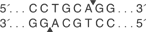
\includegraphics[scale=.5]{Sbf-I-cutsite_1_v1_000015}} }
\newglossaryentry{SbfI}{name=SbfI, description={restriction enzyme with the recognition sequence CCTGCA$\downarrow$GG} }
\newglossaryentry{XhoI}{name=XhoI, description={restriction enzyme with the recognition sequence C$\downarrow$TCGAG} }
\newglossaryentry{heterochromatin}{name=heterochromatin, description={Chromatin that remains in a highly condensed state throughout the cell cycle}}

%----------------
% Acronyms
%----------------
\newacronym{snp}{SNP}{single nucleotide polymorphism}
\newacronym{rad}{RAD}{Restriction Site associated DNA}
\newacronym{pe}{PE}{paired-end}
\newacronym{se}{SE}{single-end}
\newacronym{bp}{bp}{base pair}